\mychapter{7}{Tools}
\label{chap:tools}

\section{Trimming \label{sec:trimming}}
As the name implies, trimming is the act of trimming down reads. It's most basic application is to remove left over adapters from the reads, as in some cases these adapters can interfere with the mapping process \autoref{sec:mapping}. Similar to other steps of data processing, several tools exist to trim fastq files, some of the more common ones are listed below:\\
\begin{itemize}
\item Trimmomatic \cite{bolger2014trimmomatic}
\item CutAdapt \cite{martin2011cutadapt}
\item Trim galore \cite{krueger2015trim} - This is a wrapper of FastQC \autoref{sec:fastqc} and cutadapt, which means that it utilizes FastQC to find the quality of reads as well as the adaptors, it then uses cutadapt to trim these per the users requirements.
\end{itemize}
Trimming is often used to remove adaptors, however it is also used for `quality trimming' that is the removal of low-quality reads if they are present. This is one of the reasons why fastq files contain the read sequenced along with the quality score of that read \autoref{sec:Fastq_files}. By giving a tool a threshold of quality it can remove any reads which fall below that quality threshold. Another facet of quality trimming is the removal of reads which are too short once adaptors have been removed, though the use of this step is often very dependant on the experiment performed. For example in RNAseq we would expect to do this every time otherwise the reads would be too difficult to map accurately. In cases such as 
sBLISS trimming is also performed, however this is done for both UMIs and adaptors. Since UMIs are by definition unique, the default parameters of a trimmer would not remove these. The tools within this toolbox account for this, this statement simply illustrates the thought process sometimes required to use a trimming tool.\\
For pipelines which do not come equipped with a preferred trimmer, this toolbox will favour the use of Trimmomatic due to having prior experience with the tool. For convenience, the Trimmomatic set-up in the pipelines will simply look for all known adapters, this decision was made to limit the amount of parameters a user would have to input, in this case a user does not need to know the specific adapters used for their data. Looking for all adaptors should not impact the data in any negative way as all adapters are designed to not be `seen' as known DNA sequences.

\section{Mapping \label{sec:mapping}}
Mapping is the process of determining the location of a read on the genome, thus associating reads to specific genomic elements, and eventually specific genes. In bioinformatics we have several tools for this, some of the more commonly used ones are listed below:
\begin{itemize}
\item Burrows-Wheeler Aligner, BWA for short \cite{bwa1,bwa2}
\item Bowtie2, which also utilizes the Burrows-Wheeler approach \cite{bowtie2}
\item HISAT2 (hierarchical indexing for spliced alignment of transcripts), which is more commonly used to generate RNAseq count data \cite{hisat}
\item START (Spliced Transcripts Alignment to a Reference) is another commonly used aligner for RNAseq count data \cite{star}
\end{itemize}
The above listed are but a selection of the aligners available. As can be seen aligners usually have a specialization, where BWA and Bowtie are most often used for data where genomic location, in addition to exons, are of interest. While other aligners designed for RNAseq in mind, focus on spliced (exonic) transcript alignment. There is much debate in regards to which alignment is best, and ultimately the best aligner will depend on the experimental need.\\
This toolbox will prioritize the use of the aligner specified by a pipeline. For example the authors of the sBLISS protocol use BWA, therefore this toolbox also utilizes BWA for that protocol. However for standard Chip-seq and ATAC-seq the toolbox uses Bowtie2 due to it's familiarity.\\
For the RNAseq pipeline STAR is used, again this is simply due to the author's familiarity with it.\\
Musich et. al. wrote a small review comparing some of the aligners above from the point of view of a biologist \cite{musich2021comparison}, it may be an interesting read to some.

\subsection{Genome reference files}
Genome reference files are usually found as `.fa' files. These are usually downloaded from a GRC (Genome Reference Consortium). For example the most up to date murine and human genomes can be found at Gencode (\url{https://www.gencodegenes.org/}). These files are relatively large and it would be computationally demanding to utilize them as they are, for this purpose modern mappers require that the downloaded `.fa' files be indexed before mapping. This often involves a simple command line execution, however users of this guide need not worry about it unless their desired reference genome is not include. For a list of included reference genomes see \autoref{subsec:included_genomes}.\\
The purpose of indexing is that it splits up the reference file and allows the tool to only load segments at a time instead of the entire file. Note that each tool has their own version of indexing. They are relatively similar however they do require that indexing be performed using their tool. For example, the indexes generated by bowtie2 will not be compatible with BWA. Since Bowie2, BWA, and STAR are aligners used within this pipeline, below are the three methods of generating gene indexes for each aligner respectively.

\begin{itemize}
\item Bowtie2
\begin{lstlisting}
bowtie2-build path/to/reference.fa --name pick_name
\end{lstlisting}
\item BWA
\begin{lstlisting}
bwa index path/to/reference.fa
\end{lstlisting}
\item STAR
\begin{lstlisting}
STAR --runThreadN 6 \
--runMode genomeGenerate \
--genomeDir target_directory \
--genomeFastaFiles path/to/reference.fa \
--sjdbGTFfile path/to/gene_annotation.gtf \
--sjdbOverhang 99
\end{lstlisting}


\end{itemize}

\subsection{Included genomes \label{subsec:included_genomes}}
This toolbox includes many reference genomes:\\
\begin{itemize}
\item GRCh38 - Human
\item GRCm38 - Mouse
\item WBcel235 - Celegans
\item R64-1-1 - Saccharomyces cerevisiae (Yeast)
\item Rnor\_6.0 - Rat
\item TAIR10 - Arabidopsis Thaliana
\item BDGP6 - Drosophila melanogaster
\item Ecoli
\end{itemize}
Note that additional genomes can be added upon request.\\
\todo{T2T?}
\subsection{Blacklisted regions \label{subsec:blacklisted_regions}}
An important element to Chip-seq and other associated technologies is to account for blacklisted regions. For this we specifically refer to the work carried out by ENCODE \cite{amemiya2019encode}. They define their blacklisted regions as "a comprehensive set of regions which have anomalous, unstructured, or high signal in next-generation sequencing experiments independent of cell line or experiment". They claim that the removal of these regions is an essential quality control measure. Genomes with blacklisted regions are the following:\\
\begin{itemize}
\item HUMAN (hg38)
\item HUMAN (hg19)
\item MOUSE (mm10)
\item MOUSE (mm9)
\item WORM (ce11)
\item WORM (ce10)
\item FLY (dm6)
\item FLY (dm3)
\end{itemize}
All of these files are contained in the toolbox. They can also be downloaded here (\url{https://github.com/Boyle-Lab/Blacklist/tree/master}).\\
Since these blacklists do not exist for all genomes users would have to be aware of this absence of quality control if they utilize a genome for which a blacklist is not available. Importantly this is only required for Chip-seq and Chip-seq derived methods. RNAseq would be exempt from this filtering as the blacklisted regions do not correspond to exonic areas of the genome, therefore the captured mRNA would not map to blacklisted locations. The authors also showed that blacklisting is not productive for WGS.\\
Importantly, the elements of this toolbox handles the removal of blacklisted elements in the analysis sections of the pipelines. This choice was made to clearly show the users that this step is occurring and it makes it easier to exclude this filtering step. This may be required if one is studying protein coding genes in unmappable regions of the genome as these regions would removed by the blacklist.

\section{Sorting with Samtools \label{sec:samtools}}
Samtools is a toolbox of it's own, one that is used to interact with high-throughput sequencing data \cite{li2009sequence}. One of the main functions of Samtools is called `sort', which as the name describes it allows us to sort the aligned BAM files in different ways. Another important function, and the one we focus on in this text, is `view'. The primary use of `view' is to convert a SAM file into a BAM file (see \autoref{chap:File_types}) however it also allows us to select for a quality metric called MAPQ \autoref{sec:MAPQ}. It is common for tools to select for aligned reads above a certain quality metric. In this toolbox if a quality metric has been selected the resulting file (a bam file) will carry a name indicating the threshold that was used, for example `test\_file\_q\_60.bam' which would indicate that a value of 60 was used for the filter. To better understand what these values represent see \autoref{sec:MAPQ}. By default some tools of this toolbox may use the quality threshold version, however a non-quality filtered bam file is also produced in the event that a user may prefer that output.

\section{Peak Calling \label{sec:peak_call}}
Peak Calling is a means to identify areas of the genome which have been enriched in aligned reads. The main tool used for peak calling is MACS, which now has three variations MACS1 to 3. This toolbox uses the MACS3 \cite{MACS3}.\\
MACS stands for `Model-based Analysis for ChiP-Seq'. It was initially developed for the analysis of ChiP-Seq data however it can be used in ChiP-Seq derived protocols, however it's use may be different depending on the variant. For example, MACS offers a very convenient comparison function where a `treatment' along with a control can be provided, from this it can identify peaks relevant to the `treatment' provided. However in the case of sBLISS, which contains many more hits along the genome than a traditional Chip-Seq analysis, the control-treatment comparison often fails. In these cases it is best to simply run MACS on the treatment sample and do the comparison with the control during the data analysis step.\\
When MACS is used without a control, what it identifies changes. One could say that it identifies statistically significant peaks. The wording they use is: \textit{finding significant reads coverage than (compared to) the random background.}\\
MACS is a relatively diverse tool which allows for a variety of functions however in this tool box we focus on the `callpeak' function. The tutorial and documentation can be found here (\url{https://macs3-project.github.io/MACS/docs/Advanced_Step-by-step_Peak_Calling.html}) and here (\url{https://macs3-project.github.io/MACS/docs/callpeak.html}) respectively.\\
The input file for peak calling is often a .bam file with it's associated .bai file (see \autoref{sec:BAM_files}) however it can utilize other file types. Within the context of this toolbox all uses will be done using .bam files. This represents a fastq file that has been mapped.\\
MACS3 produces a variety of results, but the one that is particularly interesting is the `narrowPeak' output. The column names can be seen in \autoref{fig:MACS3_output}. 
\begin{figure}
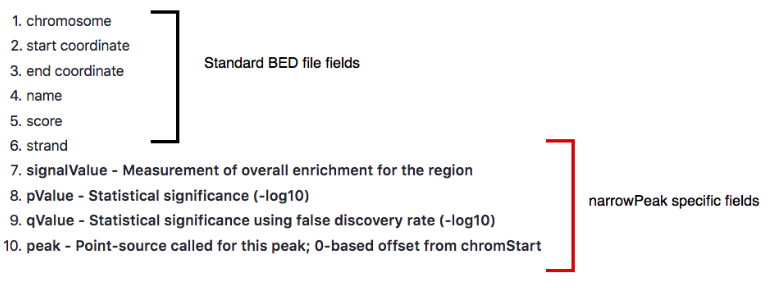
\includegraphics[width=\textwidth]{figures/MACS3_peakcall_output.png}
\caption{The output format for peak (narrow) calling using MACS3. It is found as a `.bed.narrowPeak' file extension.}
\label{fig:MACS3_output}
\end{figure}
For those interested there is a detailed guide on peak calling found here (\url{https://hbctraining.github.io/Intro-to-ChIPseq/lessons/05_peak_calling_macs.html}. It covers some important parameters and details on how peak calling works. One of these is highlighted below due to it's importance in experimental design and impact on biological interpretation.

\subsection{Understanding duplicates \label{subsec:MACS3_dups}}
In MACS3 there is a parameter called -{}-keep-dup which allows the user to keep or remove duplicates. This brings up a relevant biological question as to what is a duplicate in the context of peak calling and why these may be good or bad. For MACS a duplicate is a read which appears in the same location (in both strand and chromosomal coordinates). By default it preserves one instance per strand, though all duplicates can be preserved if desired. To better understand this we first need to understand what are good and bad duplicates. In brief: \\
\begin{itemize}
\item Good duplicates: In some biological cases one could expect many hits in similar or identical coordinates. This is particularly true in Chip-seq if the targetted protein only binds to a few sites. In this case, if you have a good amount of biological replicates, preserving duplicates is important as if they are not kept it may lead to an under-representation of the results.
\item Bad duplicates: Biases in PCR may lead to bad duplications, or in other words, artificially enriched regions, this may occur if the initial starting material (pre-PCR) is low. One may also need to be wary of blacklisted regions, that is regions which are known to produce large amounts of duplicates. To handle both of these issues one can remove duplicates. 
\end{itemize}
In the event where only blacklisted regions are a concern these can be filtered out in some steps of the pipeline. I prefer to filter them in the analysis step of the pipeline, similar to what is seen in the SBLISS PIPELINE STEP OF BLACKLIST \todo{don't forget this ref}.\\
Another method of avoiding bad duplicates is to leverage UMIs. In some protocols such as sBLISS \autoref{chap:BLISS_sBLISS} there are UMIs, where a duplicated UMI would represent a bad duplicate, while if the UMIs are different, but their location is the same, they would be good duplicates.\\
\textbf{In general, best practice is to follow the default behaviour of the pipeline, which is to remove duplicates.}


\section{Counting features \label{sec:featureCounts}}
In the case of RNA sequencing we `count' the number of reads aligned to any given gene. To do this we utilise featureCounts \cite{liao2014featurecounts}. At it's most basic featureCounts takes in a BAM file, in our case the file would be from the STAR aligner. The tool also requires an annotation file (or gtf file). The annotation file contains the name of genes, their characterization (exon, intron, ect...) as well as it's chromosomal location. In standards bulk RNAseq featureCounts will extract all exonic gene ids and match their location in the BAM file. By then counting the number of reads in that location it would obtain the number of counts for a given gene.\\
One issue that can arise between STAR and featureCounts is that the chromosome names can vary from the reference genome to the annotation file, this is largely dependant on how the reference genome was built. In our pipeline when building the STAR reference genome for GRCh38, the chromosome names ended up being swapped with GRCh38, for example chr\_1 and chr\_y became GRCh38\_1 and GRCh38\_y. Hence we adjusted the annotation file to have the same naming format. This error can be seen after an initial run of the pipeline where the `count summaries' (produced by featureCounts upon completion) states that there are many unassigned reads and 0 assigned reads, meaning none of the reads found could be matched to a location in the annotation file. If this error is observed, check the reference genomes nomenclature and verify that it matches the annotation file's nomenclature.